\documentclass[letterpaper,twocolumn,10pt]{article}
\usepackage[margin=0.75in]{geometry}

\usepackage{amsbsy}
\usepackage{graphicx}
\newcommand{\vB}{\mbox{$\bf v$}}
\newcommand{\xB}{\mbox{$\bf x$}}
\newcommand{\yB}{\mbox{$\bf y$}}
\newcommand{\JB}{\mbox{$\bf J$}}
\newcommand{\RB}{\mbox{$\bf R$}}
\newcommand{\WB}{\mbox{$\bf W$}}
\newcommand{\PB}{\mbox{$\bf P$}}
\newcommand{\MB}{\mbox{$\bf M$}}
\newcommand{\IB}{\mbox{$\bf I$}}
\newcommand{\SG}{\mbox{$\boldsymbol \Sigma$}}
\newcommand{\sG}{\mbox{$\boldsymbol \sigma$}}
%\newcommand{\SG}{\mbox{$\bf \Sigma$}}
%\newcommand{\sG}{\mbox{$\bf \sigma$}}
\newcommand{\etal}{{\em et al}}
\begin{document}

\title{\bf 
Simple FEMs aren't as good as we thought: \\
  experiences developing EIDORS v3.3%
}

\author{Andy Adler$^{1}$,
        Andrea Borsic$^{2}$,
        Nick Polydorides$^{3}$,
        William R B Lionheart$^{4}$}
\date{}
\maketitle

\renewcommand{\baselinestretch}{0.9} \normalfont
{\small \bf %
{\em Abstract --}
In this paper, we 1: announce
EIDORS version 3.3, and clarify the new features and
changes to the software.
Briefly, the new version includes:
a) interfaces to FEM generation (distmesh, netgen) and 
  dual model solvers,
b) new algorithms (total variation, electrode movement solver,
  temporal solvers),
c) a data repository with {\em in vivo} and simulated 
   data and models,
d) faster algorithms with better caching, and
e) improved graphics and extensive tutorials.
2: we review the use of dual models in EIT, and the
architecture to support their use in EIDORS.
3: we discuss accuracy limitations to the single-order
tetrahedral finite element models that are used
in much EIT research. We recommend that
models be used of at least $10^4$ elements (for 2D FEMs)
and $10^6$ elements (for 3D FEMs).
FEM accuracy may be partially addressed using
dual model solvers, for which EIDORS v3.3
provides support.
}
~\\

{\small
\noindent
$^1$Systems and Computer Engineering, Carleton University, Ottawa, Canada
$^2$Thayer School of Engineering, Dartmouth College, Hannover, NH, USA
$^3$School of Engineering, Massachusetts Institute of Technology, Boston, USA
$^4$School of Mathematics, University of Manchester, UK
}
\renewcommand{\baselinestretch}{1.0} \normalfont


\section{Introduction}

We address three issues in this paper.
First, we announce
release version 3.3 of EIDORS (Electrical Impedance Tomography and
 Diffuse Optical Tomography Reconstruction Software),
and report on the new features and their use. One significant
addition is a repository for contributed experimental 
(physiological and phantom) and
clinical data and FEM models, which we document here.

Next, we review the formulation of image reconstruction based
on dual models, in which a refined fine FEM (finite element
model) is used for the forward model, and a
coarse mesh (not necessarily based on FEM) is used of image
reconstruction. Dual models have been used in many EIT algorithms;
we review their use, and provide an algorithmic framework
to describe their application. EIDORS v3.3 provides an
architecture to support general variations of dual models,
which we describe.

Third,
since dual models are designed to allow use of large
FEMs for forward modelling, we explore the accuracy of the
first order tetrahedral models that are most commonly used
in EIT research.
We report our experience that
   simple (tetrahedral first-order) finite element models (FEMs)
      aren't as good as is generally assumed in EIT research.
Our tests show that models with less than $2,500$ elements (2D) and
$150,000$ elements (3D) are not able to reproduce the accuracy of
tank phantom measurements.
This effect is particularly severe in 3D FEM models, because
the number of elements required to achieve a given element
minimum dimension is larger by a power of $\frac{3}{2}$.
 

\section{EIDORS version 3.3}

EIDORS (Electrical Impedance Tomography and Diffuse Optical
 Tomography Reconstruction Software) is an open source
suite of software for reconstruction of images in soft 
field tomography modalities. The earliest
 version\cite{lionheart1999} was made available in 1999
and provided support for 2D EIT (documented in
\cite{vauhkonen2001}).
Subsequently, support for 3D EIT was provided\cite{polydorides2002} in 
2002. In 2005, a software refactoring was performed on the
EIDORS software base to allow ``pluggability''
-- easy incorporation of contributed algorithms and 
functionality -- as part of EIDORS version 3 (while the
previous releases were renamed v1 and v2, respectively). 
This provides many of the key features of object oriented
software, which helps to structure such large software projects.
Version 3.0 was released in 2005\cite{adler2005},
 v3.1 in 2006 (and described
in \cite{adler2006}), v3.2 in 2007, and v3.3
(described in this paper). Many new features have been added;
in terms of lines of code, v2.0 has 3715, v3.0 has 10685
and v3.3 has $22424$ (with another $11705$ in tutorials).

The following high-level new features are part of EIDORS v3.3:

\newcounter{Ictr}
\begin{list}{\bf \arabic{section}.\arabic{Ictr}}
  {\leftmargin=0.0em \itemindent=2.0em
%   \topsep= 0.0\baselineskip
%   \itemsep=-0.0em
    \listparindent=1.0em \parsep=-0.0em
    \usecounter{Ictr}}
\item {\bf Interfaces to FEM generation tools:} \\
(Netgen\cite{schoeberl1997}
and Distmesh\cite{persson2004})

\item {\bf Support for dual model solvers:}

\item {\bf New reconstruction algorithms:}
 total variation, electrode movement solver,
  temporal solvers

\item {\bf Data repository:}
 with several contributed models, clinical
   and experimental data sets

\item {\bf Faster algorithms:} for calculation of
   Total Variation PDIPM, Jacobian; better caching;
   an iterative forward solver (to save memory, if required)

\item {\bf Improved graphics and extensive tutorials}

\end{list}

\section{Data Repository}

EIDORS incorporates a data repository which includes
animal and clinical experimental EIT data
(including the earliest EIT measurements\cite{barber1983}), 
calibrated phantom data, and FEM models and
simulation data. The goal of the EIDORS data
repository is to: 
1) allow new researchers in the community to have some real data against
which they can test their software, and
2) allow testing of algorithms against available and standard benchmark data.

Licensing of contributed data depends on the choice of
the owners of each contribution. The 
default license is the Creative Commons Artistic License
(with attribution). This license allows copying, distribution, and
derivative works with the requirement that the user give the
author credit as specified. 
Generally, contributed data forms part of a published
study, and the credit requirement is fulfulled by 
referencing the original study.


\begin{figure}[tbh]
\begin{center}
 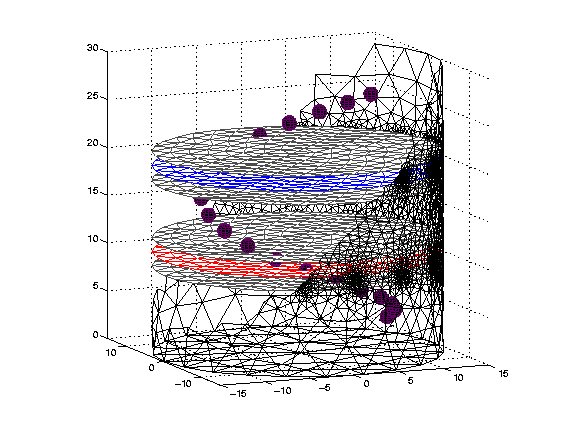
\includegraphics[width= 0.45\textwidth]{../../tutorial/dual_model/centre_slice02a.png}
\caption{ \label{fig:dual_model}
\small
Netgen model of a $2\times 16$ electrode tank. The positions of the simulated
conductive target moving in a helical path are shown in purple. The
3D fine model is shown (cropped). The upper (blue) and lower (red)
layers corresponding to the geometry of the coarse model are shown. The
$z$-direction limits of the coarse model are shown in grey.
}
\end{center}
\vspace{-1cm}
\end{figure}

\begin{figure}[tbh]
\begin{center}
 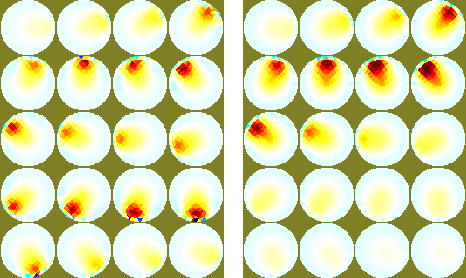
\includegraphics[width= 0.45\textwidth]{figs/centre_slice04a_crop.png}
\caption{ \label{fig:dual_model_reconst}
\small
Reconstructed images of a target moving in a helical pattern using
difference reconstruction models.
{\em Left} reconstruction model with  $z_{depth}=\infty$
{\em Right} reconstruction model with $z_{depth}= 0.1\times \mbox{scale}$
at lower position in Fig.~\ref{fig:dual_model}
}
\end{center}
\vspace{-0.5cm}
\end{figure}

\section{Dual Model solvers}


A dual reconstruction model uses a high density (fine)
FEM to implement the forward solution (voltages
at electrodes), and a low density (coarse) mesh
(not necessarily FEM based) for the inverse
solution. For example, a dual model may be used to 
represent the conductivity change in a layer
of a 3D plane (Fig.~\ref{fig:dual_model}).
Given a forward model, $F$,
which calculates a voltage measurement vector, $\vB$, from
a forward (fine) model conductivity element vector, $\sG_f$, we
have $\vB = F( \sG_f )$. The reconstruction (coarse)
model is defined on square elements $\sG_r$ related by
a coarse to fine projection matrix $\PB$, where $\sG_f = \PB \sG_r$.

This is implemented in EIDORS as follows. For each
inverse model, represented as part of the {\tt inv\_model}
structure (Fig.~\ref{fig:invmdl}),
there are two {\tt fwd\_model} structures:
1) the refined forward model {\tt fwd\_model}, and
2) the reconstruction model {\tt rec\_model}. 
Within each forward model structure is a matrix field
{\tt coarse2fine} which is a sparse encoding of $\PB$.
Each element $[\PB]_{i,j}$ represents the fraction of
fine element $i$ enclosed within coarse element $j$.

The Jacobian matrix may be defined for the coarse
($\JB_r$) and fine ($\JB_f$) models as follows:
\begin{equation}
\vB = \JB_f \sG_f 
    = \JB_f \PB \sG_r
    = \JB_r     \sG_r
\end{equation}
and thus $\JB_r = \JB_f \PB$. Since the matrix
$\JB_f$ is very large, EIDORS will not calculate it
directly. Instead, an efficient algorithm calculates
each column of $\JB_r$ using
\begin{equation}
\big[ \JB_c \big]_{i,j} =
\big[ \JB_f \PB \big]_{i,j} =
\sum_k \frac{\partial [ \vB ]_i }
            {\partial [ \sG_f ]_k } [\PB]_{k,j}
= \frac{\partial [ \vB ]_i }
       {\partial [ \sG_c ]_j }
\end{equation}
where the last expression is implemented in terms
of the FEM system matrix using the adjoint field method.

The need for a matrix $\PB$ on the {\tt rec\_model} is
due to the limits of the first order FEM representation.
If the regions in the reconstruction model are not
triangular, then each region is constructed from triangular
regions and the parametrization represented in $\PB$.

\begin{figure}[tbh]
\begin{center}
 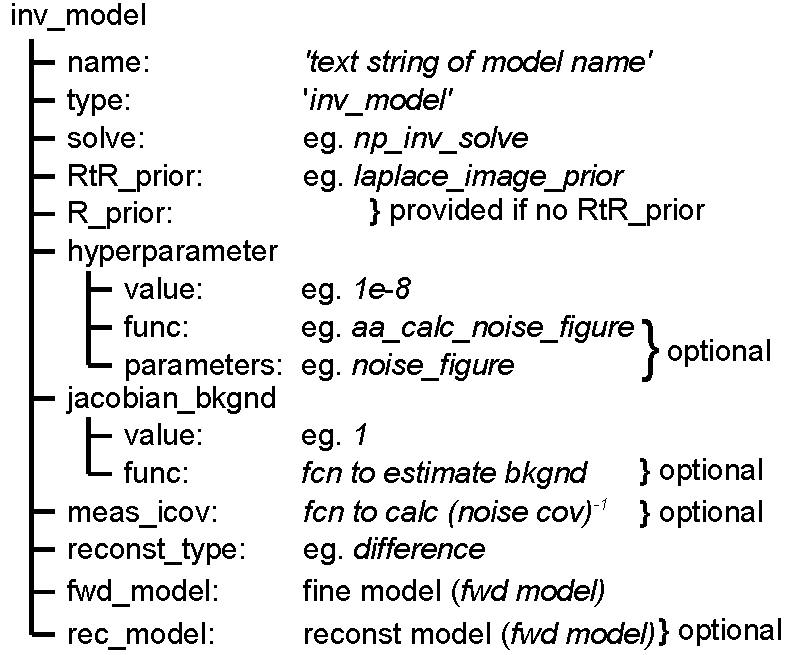
\includegraphics[width= 0.40\textwidth]{figs/inv_model.png}
\caption{ \label{fig:invmdl}
\small
Layout of the EIDORS {\tt inv\_model} object
}
\end{center}
\vspace{-0.5cm}
\end{figure}

Dual meshes may be used in several applications:
\begin{list}{$\circ$} %{\textbullet}
  {\leftmargin=1.0em \itemindent=-0.0em
    \topsep=0.0\baselineskip
    \itemsep=-0.4\baselineskip}
\item
   Corresponding meshes: where 
   coarse elements completely contain fine ones but do not
   cross elements.
\item
   Nodal Solvers: in which the reconstruction parameterizes
   the conductivity on each node\cite{graham2006}.
\item
   $2\frac{1}{2}$D Solvers: in which the $z$-dimension of the
     3D fine model is projected onto a 2D reconstruction model.
     This technique is widely used in geophysical appications.
\item
   Constraining Reconstruction Parameters:
      this is useful for example to have one parameter
      for out of plane conductivity (a region of low sensitivity),
      which may prevent the algorithm from ``pushing" artefacts there.
\item
   Solving to a Square Pixel Grid: this is useful because the
       reconstructed image is typically mapped to pixels, and
       will often show artefacts based on the shapes of the elements.
       A rasterized reconstruction grid will prevent such
       artefacts, and allow more natural communication of the
       underlying system resolution (via the pixel size).
\end{list}


%Dual meshes have been used by many EIT groups
%\\
%- Oxford Brookes used an interpolation method on two meshes since the early code in the Fortran code Recon started by Lionheart and continued by Kevin Paulson at Brookes. The approach used a mesh correspondence array. 
%\\
%- Later on the Dartmouth group also used the idea; paper by the
%   similarly named Keith Paulsen (ref).
%\\
%- Marko Vauhkonen use two meshes in the original 2D EIDORS.
%\\
%- UCL optimal tomography group uses it for TOAST.
%
\begin{figure}[tbh]
\begin{center}
 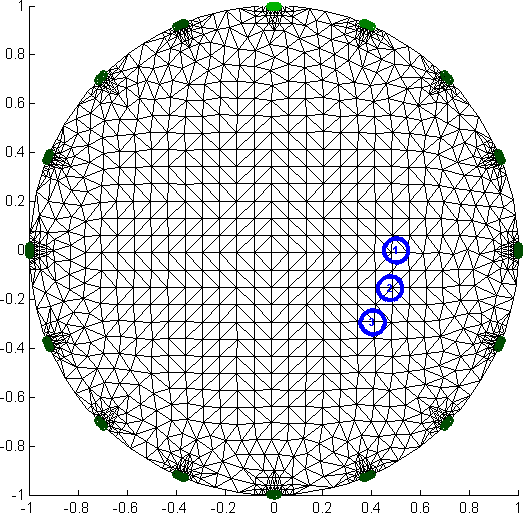
\includegraphics[width= 0.24\textwidth]{figs/fig1a.png}
 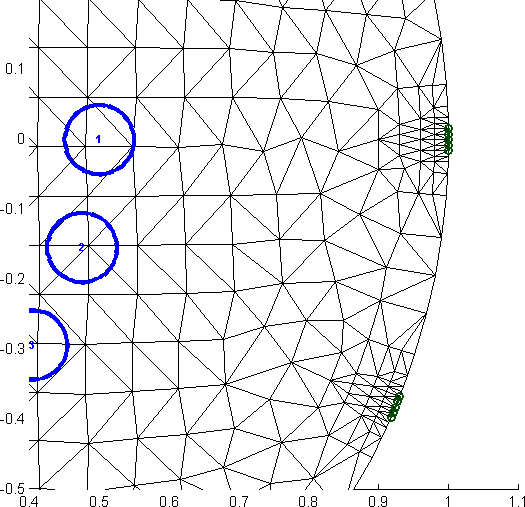
\includegraphics[width= 0.24\textwidth]{figs/fig1b.png}
\caption{ \label{fig:fem1}
\small
Simulation FEM and simulated target positions in blue
{\em Left} full scale mesh.
{\em Right} mesh magnified near target positions 
}
\end{center}
\vspace{-1.0cm}
\end{figure}

\section{FEM accuracy}

Finite Element Model accuracy is normally considered
from the point of view of voltage errors between FEM and
physical phantom. While this is correct, any errors may be explained
by small details in the phantom which are not considered
in the model. This means that it is difficult to use such
a test to verify high model accuracy, which is necessary
in a soft field tomography modality.
Instead, we consider FEM accuracy by
looking at small changes in the model and the
consequences on difference EIT images.

\begin{figure}[tbh]
\begin{center}
 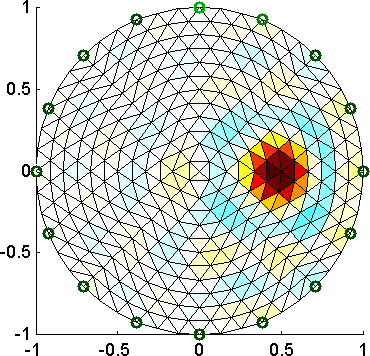
\includegraphics[width= 0.15\textwidth]{figs/fig2a.png}
 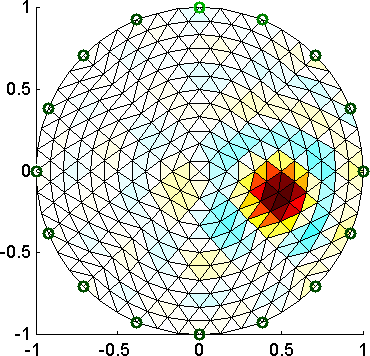
\includegraphics[width= 0.15\textwidth]{figs/fig2b.png}
 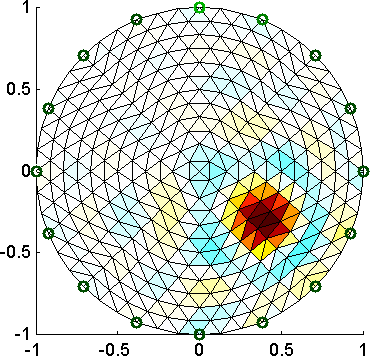
\includegraphics[width= 0.15\textwidth]{figs/fig2c.png}
\caption{ \label{fig:fem1_images}
\small
Images reconstructed from simulations 
interpolating shapes in Fig. \ref{fig:fem1}; from
left to right, targets 1 to 3. No model noise
is seen in the images.
}
\end{center}
\vspace{-0.5cm}
\end{figure}

The easiest (and most common) way to simulate a moving target
in a medium is to use a single FEM to select and then interpolate
which elements are part of that target. There is no change to
the underlying FEM, and thus no model noise in the images.

To illustrate this process, Fig.~\ref{fig:fem1}
shows two 2372 element FEMs created by distmesh, with mesh
refinement near the electrodes. Electrodes are
simulated using a Sheffield-type adjacent stimulation and
measurement. For each simulated target position (blue), the
fraction of each element filled by the target is calculated
and used to scale the simulated conductivity change in the element.
Images are reconstructed of the three target positions
in Fig. \ref{fig:fem1_images} using a one-step regularized
GN image reconstruction. No noise is seen from the simulation,
as expected, since the FEM model does not change.

However, the most appropriate way to simulate a moving target is
create a target region within the FEM and to remesh around
it. This means that the mesh changes between each
target position, not only near the target, but throughout
the FEM due to the propagation of changes in triangularization.

\begin{figure}[tbh]
\begin{center}
 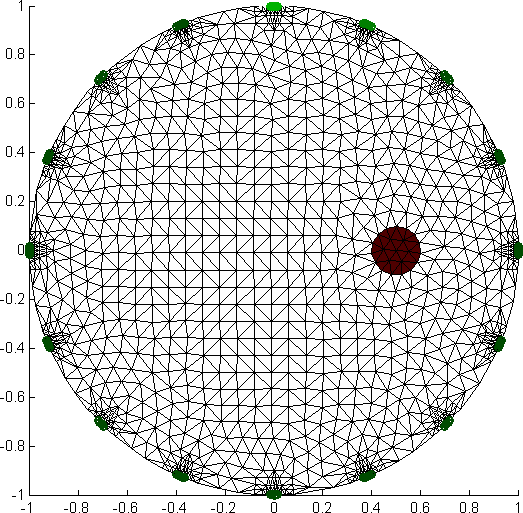
\includegraphics[width= 0.24\textwidth]{figs/fig3a-2372e.png}
 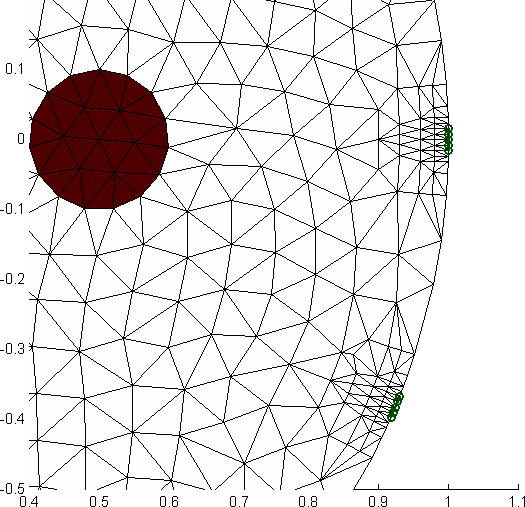
\includegraphics[width= 0.24\textwidth]{figs/fig3b-2372e.png}
 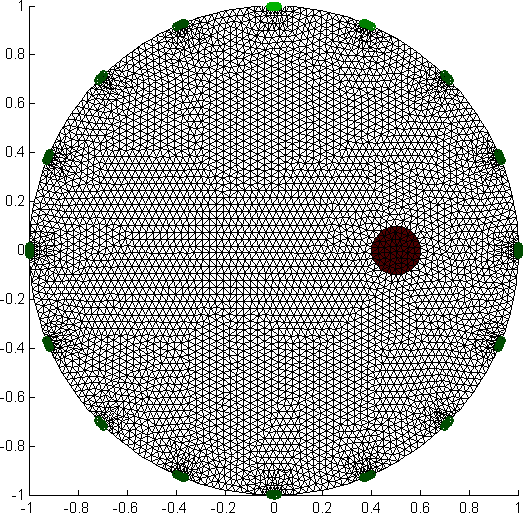
\includegraphics[width= 0.24\textwidth]{figs/fig3a-8909e.png}
 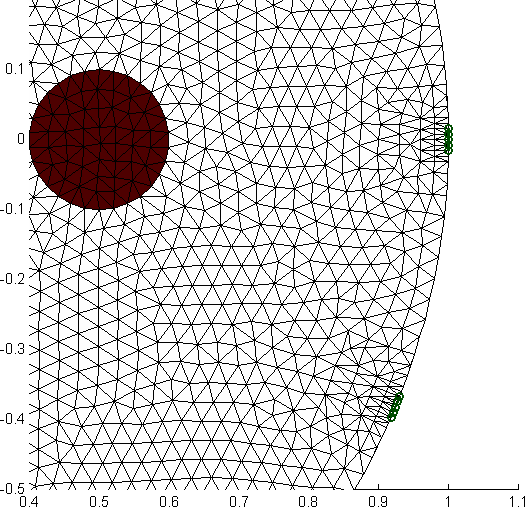
\includegraphics[width= 0.24\textwidth]{figs/fig3b-8909e.png}
\caption{ \label{fig:fem2}
\small
Simulation FEM and simulated target positions in blue
{\em Left} full scale mesh.
{\em Right} mesh magnified near target positions 
{\em Top} FEM with 2372 elements,
{\em Bottom} FEM with 8909 elements,
}
\end{center}
\vspace{-0.5cm}
\end{figure}

Using distmesh\cite{persson2004},
 FEMs were created of a homogeneous phantom
(like that of Fig. \ref{fig:fem1}), and of three phantoms
with inset targets areas in the corresponding positions.
Fig. \ref{fig:fem2} shows the mesh at the
first target position. Three different levels of mesh
refinement are shown.

Based on these simulations, we reconstruct images
using a simple 576 element reconstruction model with point electrodes
(Fig.~\ref{fig:fem2_images}). In the coarse (2372 element)
and to a lesser extent in the refined (8909 element) 
mesh, there are artefacts, mostly near the electrodes, which
dramatically disturb the image clarity.

\begin{figure}[tbh]
\begin{center}
 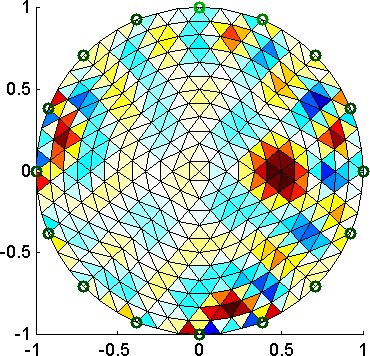
\includegraphics[width= 0.15\textwidth]{figs/fig4a-2372e.png}
 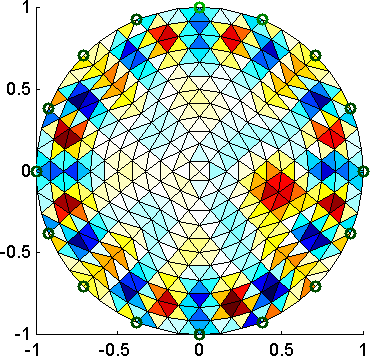
\includegraphics[width= 0.15\textwidth]{figs/fig4b-2372e.png}
 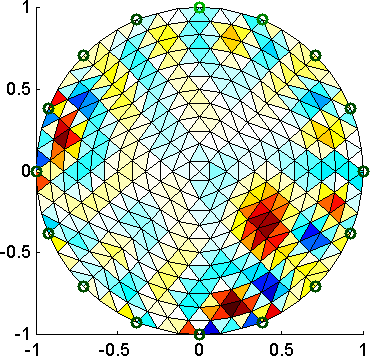
\includegraphics[width= 0.15\textwidth]{figs/fig4c-2372e.png}
 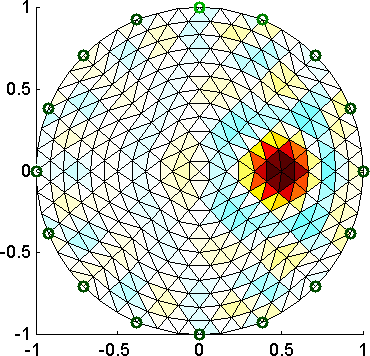
\includegraphics[width= 0.15\textwidth]{figs/fig4a-8909e.png}
 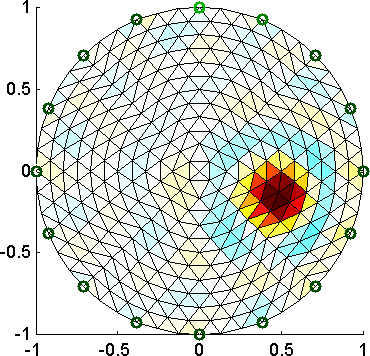
\includegraphics[width= 0.15\textwidth]{figs/fig4b-8909e.png}
 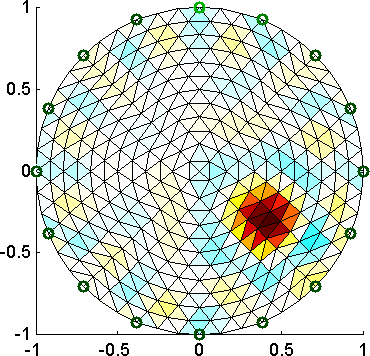
\includegraphics[width= 0.15\textwidth]{figs/fig4c-8909e.png}
\caption{ \label{fig:fem2_images}
\small
Images reconstructed of targets simulated from
interpolated shapes in Fig. \ref{fig:fem2}, from
left to right, targets 1 to 3.
{\em Top} FEM with 2372 elements,
{\em Bottom} FEM with 8909 elements,
}
\end{center}
\vspace{-0.5cm}
\end{figure}

\begin{figure}[tbh]
\begin{center}
 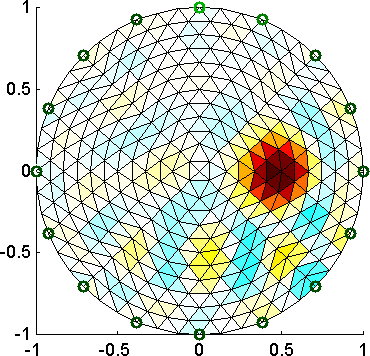
\includegraphics[width= 0.15\textwidth]{figs/fig5a.png}
 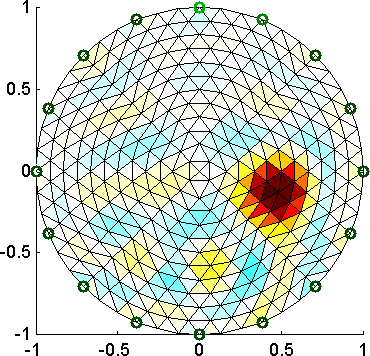
\includegraphics[width= 0.15\textwidth]{figs/fig5b.png}
 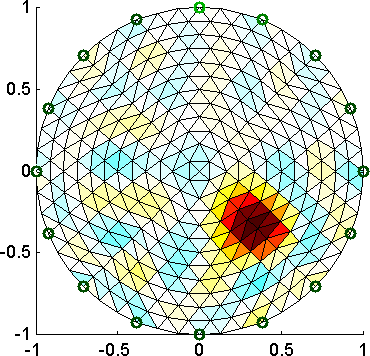
\includegraphics[width= 0.15\textwidth]{figs/fig5c.png}
\caption{ \label{fig:iirc_data}
\small
Images reconstructed of a target in a saline tank
with the same reconstruction parameters as Fig.~\ref{fig:fem2_images}.
}
\end{center}
\vspace{-0.5cm}
\end{figure}

To compare with these images, a sequence of EIT
data were gathered with a 16 electrode system from
the IIRC from Kyung Hee University, Korea. A saline
filled tank was used and a small non-conductive target
was slowly rotated around the tank. Frames of data
corresponding to the simulated positions are shown.
Images are reconstructed from these data using the
same reconstruction parameters and shown in
Fig.~\ref{fig:iirc_data}. These images show some artefacts
in the lower part of the image (probably due to waves
in the tank from the movement), but show less of the
artefacts (near the electrodes)
seen in Fig.~\ref{fig:fem2_images}.

\begin{figure}[tbh]
\begin{center}
 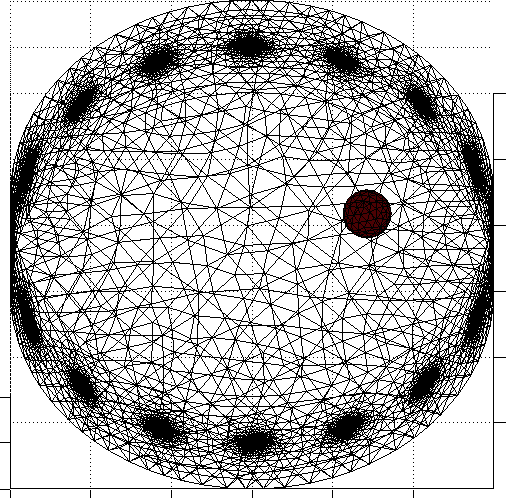
\includegraphics[width= 0.20\textwidth]{figs/fig9a.png}
 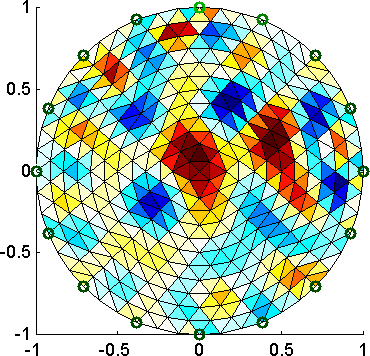
\includegraphics[width= 0.20\textwidth]{figs/fig9b.png}
\caption{ \label{fig:netgen_3D}
\small
{\em Right:}
3D models from netgen \cite{schoeberl1997}
of a moving ball in a 16 electrode tank
with $131,640$ elements.
{\em Left:}
Image reconstructed using the same parameters
in the previous figures. Significant artefacts
are shown, due to the inadequate element size.
}
\end{center}
\vspace{-0.5cm}
\end{figure}


The same effect can be seen in 3D FEM, and is even
more significant because the number of elements
required to achieve a minimum element dimension
is larger in 3D by approximately a power of $\frac{3}{2}$.
Fig.~\ref{fig:netgen_3D} shows an example of a
ball of the same radius as the 2D examples introduced
into a $131,640$ element FEM using netgen\cite{schoeberl1997}.
Significant artefacts are seen, even for a very large
model size.
We have currently not been able to generate sufficiently
large FEM models to eliminate reconstruction
artefacts, due to memory constraints on our systems.


\section{Discussion}

In this paper we: 1) announce
EIDORS version 3.3, and clarify the new features and
changes to the software;
2) review the use of dual models in EIT, and
the architecture to support their use in EIDORS;
and
3) discuss the accuracy limitations to the single-order
tetrahedral finite element models that are used
in much EIT research. As a preliminary recommendation,
we suggest a minimum model size of $10^4$ elements
 (2D FEM) and $10^6$ (3D FEM).

\begin{thebibliography}{1}
\setlength{\parskip}{0ex}%
\setlength{\itemsep}{0ex}%
\small%
%
\bibitem{adler2006}
Adler A and
Lionheart WRB
(2006)
Uses and abuses of EIDORS: An extensible software base for EIT.
\emph{Physiol. Meas.}
27:S25--S42
%
\bibitem{adler2005}
Adler A and
Lionheart WRB
(2005)
EIDORS: Towards a community-based extensible software base for EIT
{\em Conf. Biomedical Applications of EIT}
London, UK, June 22-24
%
\bibitem{barber1983}
Barber BC
Brown BH and
Freeston IL,
(1983)
Imaging spatial distributions of resistivity using
applied potential tomography,
{\em Electronics Let},
19:933--935
%
\bibitem{graham2006}
Graham B and Adler A,
(2006)
A Nodal Jacobian Algorithm for Reduced Complexity EIT Reconstructions
{\em Int. J. Inform. Systems Sciences},
2:453--468.

\bibitem{lionheart1999}
Lionheart WRB,
Arrridge SR,
Schweiger M,
Vauhkonen M and
Kaipio JP
(1999)
Electrical Impedance and Diffuse Optical Tomography
Reconstruction Software
{\em World Congress Indust.\ Proc.\ Tomog.\ },
Manchester, UK, April 14-17

\bibitem{persson2004}
Persson P-O and
Strang G
(2004)
A Simple Mesh Generator in MATLAB
{\em SIAM Review}
46:329--345

\bibitem{polydorides2002}
Polydorides N and
Lionheart  WRB
(2002)
A Matlab toolkit for three-dimensional electrical impedance tomography:
a contribution to the Electrical Impedance and Diffuse Optical
Reconstruction Software project
{\em Meas. Sci. Technol.}
13:1871--1883 

\bibitem{schoeberl1997}
Sch\"oberl J
(1997)
NETGEN: An advancing front 2D/3D-mesh generator based on
abstract rules
{\em Comput.\ Visual.\ Science}
1:41--52

\bibitem{vauhkonen2001}
Vauhkonen M,
Lionheart WRB,
Heikkinen LM,
Vauhkonen PJ and
Kaipio JP
(2001)
A MATLAB package for the EIDORS project to reconstruct two-dimensional EIT 
images
{\em Physiol Meas}
22 107-111

\end{thebibliography}
\end{document}

